\documentclass[../main.tex]{subfiles}
\graphicspath{{\subfix{../images/}}}
\begin{document}
\section*{Term 1 Week 9}
\begin{enumerate}
    \item 
    Solve for \(x\):\\
    \[\frac{1}{\log_8(x)}+\frac{1}{\log_x(\frac{1}{4})}=-\frac{5}{2}\]\\

    \item 
    Water leaks out of a cylindrical tank through a small hole at the base at a rate proportional to the square root of the depth.\\
    
    Initially the tank is full. After one hour, it is half-empty. How much time will it take to empty the tank completely?\\
    \begin{figure}[h]
        \centering
        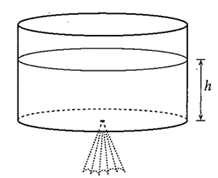
\includegraphics{images/t1w9q2.png}
    \end{figure}\\

    \item 
    Consider the function \(y=\frac{1}{\sqrt{2\pi}}e^{-\frac{x^2}{2}}\). This is commonly called the \textit{standard normal curve}.\\

    Consider the tangents to the steepest points on the standard normal curve.\\
    
    Show that these tangents and the x-axis enclose a triangular area equal to \(\sqrt{\frac{8}{\pi e}}\)
    \begin{figure}[h]
        \centering
        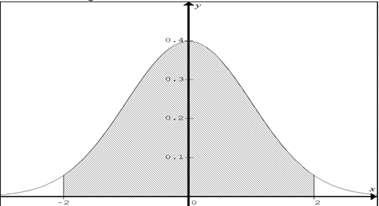
\includegraphics[width=0.5\linewidth]{images/t1w9q3.png}
    \end{figure}
    
\end{enumerate}

\end{document}